%%%%(c)
%%%%(c)  This file is a portion of the source for the textbook
%%%%(c)
%%%%(c)    Abstract Algebra: Theory and Applications
%%%%(c)    Copyright 1997 by Thomas W. Judson
%%%%(c)
%%%%(c)  See the file COPYING.txt for copying conditions
%%%%(c)
%%%%(c)
\chapter*{Hints and Solutions}
 
 
\addcontentsline{toc}{chapter}{Hints and Solutions}
\pagestyle{myheadings}
\markboth{HINTS AND SOLUTIONS}{HINTS AND SOLUTIONS}
 
 
 
\subsection*{Chapter 1. Preliminaries}
 
 
{\small
\begin{itemize}
 
\item[1.]
(a) $\{ 2 \}$.
(b) $\{ 5 \}$.
 
\item[2.]
(a) $\{ (a,1), (a,2), (a,3), (b,1), (b,2), (b,3), (c,1), (c,2),
(c,3) \}$. \\
(d) $\emptyset$.
 
\item[6.]
If $x \in A \cup (B \cap C)$, then either $x \in A$ or $x \in B \cap 
C$  $\Rightarrow x \in A \cup B \text{ and } A \cup C \Rightarrow x
\in (A \cup B) \cap (A \cup C) \Rightarrow  A \cup (B \cap C) \subset 
(A \cup B) \cap (A \cup C)$. 
 
Conversely, $x \in (A \cup B) \cap (A \cup C) \Rightarrow  x \in A 
\cup B \text{ and } A \cup C \Rightarrow x \in A  \text{ or } x \text{ is in
both } $B$ \text{ and } $C$  \Rightarrow x \in A \cup (B \cap C) \Rightarrow
(A \cup B) \cap (A \cup C) \subset A \cup (B \cap C)$. Hence, $A \cup 
(B \cap C) = (A \cup B) \cap (A \cup C)$. 
 
\item[10.]
$(A \cap B) \cup (A \setminus B) \cup (B \setminus A) = (A \cap B) \cup 
(A \cap B') \cup (B \cap A') = [A \cap (B \cup B')] \cup (B \cap A')
= A \cup (B \cap A') = (A \cup B) \cap (A \cup A') = A \cup B$.
 
 
\item[14.]
$A \setminus (B \cup C) = A \cap (B \cup C)'
= (A \cap A) \cap (B' \cap C')
= (A \cap B') \cap (A \cap C') = 
(A \setminus B) \cap (A \setminus C)$. 
 
\item[17.]
(a) Not a map. $f(2/3)$ is undefined. \\
(c) Not a map. $f(1/2) =3/4$ and $f(2/4)=3/8$.
 
\item[18.]
(a)  One-to-one but not onto. $f({\mathbb R} ) = \{ x \in {\mathbb R} : x
> 0 \}$. \\
(c) Neither one-to-one nor onto.
 
\item[20.]
(a) $f(n) = n + 1$.
 
\item[22.]
(a) Let $x, y \in A$. Then $g(f(x)) = (g \circ f)(x) = (g \circ
f)(y) = g(f(y)) \Rightarrow f(x) = f(y) \Rightarrow x = y$,  so $g
\circ f$ is one-to-one. \\
(b) Let $c \in C$, then $c = (g \circ f)(x) = g(f(x))$ for some
$x \in A$. Since $f(x) \in B$, $g$ is onto.
 
\item[23.]
$f^{-1}(x) = (x+1)/(x-1)$.
 
\item[24.]
(a)  Let $y \in f(A_1 \cup A_2) \Rightarrow$ there exists an $x
\in A_1 \cup A_2$ such that $f(x) = y \Rightarrow y \in f(A_1)$ or
$f(A_2) \Rightarrow y \in f(A_1) \cup f(A_2) \Rightarrow f(A_1 \cup A_2)
\subset f(A_1) \cup f(A_2)$.
 
Conversely, let $y \in f(A_1) \cup f(A_2) \Rightarrow y \in f(A_1)$ or
$f(A_2) \Rightarrow$ there exists an $x \in A_1$ or there exists an
$x \in A_2$ such that $f(x) = y \Rightarrow$ there exists an $x \in
A_1 \cup A_2$ such that $f(x) = y \Rightarrow f(A_1) \cup f(A_2)
\subset f(A_1 \cup A_2)$. Hence, $f(A_1 \cup A_2) = f(A_1) \cup f(A_2)$. 
 
\item[25.]
(a) Not an equivalence relation. Fails to be symmetric.\\
(b) Not an equivalence relation. Fails to be reflexive since 0 is not equivalent to itself.\\
(c) Not an equivalence relation. Fails to be transitive.

%Solution to (b) corrected.  Suggested by R. Nilange.
%TWJ 8/14/2013 


 
\item[28.]
Let $X = {\mathbb N} \cup \{ \sqrt{2}\, \}$ and define $x \sim y$ if $x + y
\in {\mathbb N}$.
 
\end{itemize}
}
 
 
 
\subsection*{Chapter 2. The Integers}
 
 
{\small
\begin{itemize}
 
 
\item[1.]
$S(1): [1(1+1)(2(1) + 1)]/6 = 1 = 1^2$ is true. Assume $S(k): 1^2 +2^2
+ \cdots + k^2 = [k(k+1)(2k+1)]/6$ is true. Then $1^2 + 2^2 + \cdots +
k^2 + (k+1)^2 = [k(k+1)(2k+1)]/6 + (k+1)^2 = [(k+1)((k+1) +1)(2(k+1) +
1)]/6$, so $S(k+1)$ is true. Thus $S(n)$ is true for all positive
integers $n$. 
 
\item[3.]
$S(4): 4! = 24 > 16 =2^4$ is true. Assume $S(k): k! >2^k$ is true.
Then $(k+1)! = k! (k+1) > 2^k \cdot 2 = 2^{k+1}$, so $S(k+1)$ is true.
Thus $S(n)$ is true for all positive integers $n$. 
 
 
\item[8.]
Look at the proof in Example~\ref{example:integers:binomial_theorem}.
 
\item[11.]
$S(0): (1+x)^0 -1 = 0 \geq 0 = 0 \cdot x$ is true. Assume $S(k):
(1+x)^k -1 \geq kx$ is true. Then $(1+x)^{k+1} - 1 = (1+x)(1+x)^k -1 =
(1+x)^k + x(1+x)^k -1 \geq kx + x(1+x)^k \geq kx + x = (k+1)x$, so
$S(k+1)$ is true. Thus $S(n)$ is true for all positive integers $n$.
 
 
\item[15.]
(a) $(14)14 + (-5)39 = 1$.\\
(c) $(3709) 1739 + (-650) 9923 = 1$.\\
(e) $(881) 23771 + (-1050) 19945 = 1$.
 
 
\item[17.]
(b) Use mathematical induction.
(c) Show that $f_1 = 1$, $f_2 = 1$, and $f_{n + 2}
= f_{n + 1} + f_n$.
(d) Use part (c).
(e) Use part (b) and Problem 16.
 
 
\item[19.]
Use the Fundamental Theorem of Arithmetic.
 
 
\item[23.]
Let $S = \{s \in {\mathbb N} : a \mid s$, $b \mid s \}$. $S \neq \emptyset$,
since $|ab| \in S$. By the Principle of Well-Ordering, $S$ contains a
least element $m$. To show uniqueness, suppose that $a \mid n$ and $b
\mid n$ for some $n \in {\mathbb N}$. By the division algorithm, there
exist unique integers $q$ and $r$ such that $n = mq + r$, where $0
\leq r < m$. $a \mid m$, $b \mid m$, $a \mid n$, $b \mid n \Rightarrow a
\mid r$, $b \mid r \Rightarrow r = 0$ by the minimality of $m$.
Therefore, $m \mid n$. 
 
 
\item[27.]
Since $\gcd(a,b)=1$, there exist integers $r$ and $s$ such that $ar +
bs =1 \Rightarrow acr+bcs =c$. Since $a \mid a$ and $a \mid bc$, $a
\mid c$.
 
 
\item[29.]
Every prime number greater than 3, must be of the form $6 n \pm 1$ for some $n \in \mathbb N$.
Suppose that there are only a finite number of primes of  the form $6n +1$,
\[
p_1 = 6n_1 + 1, p_2 = 6 n_2 + 1, \ldots, p_k = 6n_k + 1.
\]
Let $p = p_1 p_2 \cdots p_k + 1$.  Then $p$ must be of the form $6m + 1$ for some $m \in \mathbb N$.  Since $p$ is not divisible by any prime of the form $6 n -1$ or $p_1, p_2, \ldots, p_k$, it must be prime which contradicts the fact that the only primes of the form $6n + 1$ are $p_1, p_2, \ldots, p_k$.

%Replaced the incorrect hint with a correct solution.
%D. Keeler pointed out the error.  TWJ 1/10/2014
 
\end{itemize}
}
 
 
 
\subsection*{Chapter 3. Groups}
 
 
{\small
\begin{itemize}
 
\item[1.]
(a) $\{ \ldots, -4, 3, 10, \ldots \}$.
(c) $\{ \ldots, -8, 18, 44, \ldots \}$.
(e) $\{ \ldots, -1, 5, 11, \ldots \}$.
 
\item[2.]
(a) Not a group.
(c) A group.
 
 
 
\item[6.] 
\raisebox{-24pt}{\parbox{1.85in}{
\begin{tabular}{c|cccc}
$\cdot$ & 1  & 5  & 7  & 11 \\
\hline
1     & 1  & 5  & 7  & 11 \\
5     & 5  & 1  & 11 & 7 \\
7     & 7  & 11 & 1  & 5 \\
11    & 11 & 7  & 5  & 1
\end{tabular}
}}
 
 
\item[8.]
Pick two matrices. Almost any pair will work.
 
\item[15.]
There is a group of order 6 that is nonabelian.
 
\item[16.]
Look at the symmetry group of an equilateral triangle or a square.
 
\item[17.]
There are actually five different groups of order 8.
 
\item[18.]
Let
\[
\sigma
=
\begin{pmatrix}
1   & 2   & \cdots & n \\
a_1 & a_2 & \cdots & a_n
\end{pmatrix}
\]
be in $S_n$. All of the $a_i$'s must be distinct.  There are $n$ ways
to choose $a_1$, $n-1$ ways to choose $a_2$, $\ldots$, 2 ways to
choose $a_{n-1}$, and only one way to choose $a_n$. Therefore, we can form
$\sigma$ in $n(n-1) \cdots 2 \cdot 1 = n!$ ways.
 
\item[25.]
$(aba^{-1})^n = (aba^{-1})(aba^{-1}) \cdots (aba^{-1}) 
= ab(aa^{-1})b(aa^{-1})b \cdots (aa^{-1})ba^{-1} = ab^na^{-1}$.
 
\item[31.]
$abab = (ab)^2 = e = a^2 b^2 = aabb\Rightarrow  ba = ab$.
 
\item[35.]
$H_1 = \{ id \}$, $H_2 = \{ id, \rho_1, \rho_2  \}$, $H_3 = \{ id,
\mu_1 \}$, $H_4 = \{ id, \mu_2 \}$, $H_5 = \{ id, \mu_3 \}$, $S_3$.
 
\item[41.]
$id = 1 = 1 + 0 \sqrt{2}$, $(a + b \sqrt{2}\, )(c + d \sqrt{2}\, ) = 
(ac + 2bd) + (ad + bc)\sqrt{2}$, and $(a + b \sqrt{2}\, )^{-1} = a/(a^2
-2b^2) - b\sqrt{2}/(a^2 - 2 b^2)$.
 
\item[46.]
Not a subgroup. Look at $S_3$.
 
\item[49.]
$a^4b =ba \Rightarrow b = a^6 b = a^2 b a \Rightarrow ab = a^3 b a =
ba$. 
 
\end{itemize}
}
 
\subsection*{Chapter 4. Cyclic Groups}
 
{\small
\begin{itemize}
 
\item[1.]
(a) False.
(c) False.
(e) True.
 
\item[2.]
(a) 12.
(c) Infinite.
(e) 10.
 
\item[3.]
(a) $7 {\mathbb Z} = \{ \ldots, -7, 0, 7, 14, \ldots \}$. 
(b) $\{ 0, 3, 6, 9, 12, 15, 18, 21 \}$. \\
(c) $\{ 0 \}, \{ 0, 6 \}, \{ 0, 4, 8 \}, \{ 0, 3, 6, 9 \}, \{ 0,
2, 4, 6, 8, 10 \}$. \\
(g) $\{ 1, 3, 7, 9 \}$.
(j) $\{ 1, -1, i, -i \}$.
 
\item[4.]
(a) 
\raisebox{-6.5pt}{\parbox{4in}{
\[
\begin{pmatrix}
1 & 0 \\
0 & 1
\end{pmatrix},
\begin{pmatrix}
-1 & 0 \\
0 & -1
\end{pmatrix},
\begin{pmatrix}
0 & -1 \\
1 & 0
\end{pmatrix},
\begin{pmatrix}
0 & 1 \\
-1 & 0
\end{pmatrix}.
\]
}}

(c) 
\raisebox{-23.5pt}{\parbox{4in}{
\[
\begin{array}{c}
\begin{pmatrix}
1 & 0 \\
0 & 1
\end{pmatrix},
\begin{pmatrix}
1 & -1 \\
1 & 0
\end{pmatrix},
\begin{pmatrix}
-1 & 1 \\
-1 & 0
\end{pmatrix},\\ \\
\begin{pmatrix}
0 & 1 \\
-1 & 1
\end{pmatrix},
\begin{pmatrix}
0 & -1 \\
1 & -1
\end{pmatrix},
\begin{pmatrix}
-1 & 0 \\
0 & -1
\end{pmatrix}.
\end{array}
\]
}}
 
\item[10.]
(a) $0, 1, -1$.
(b) $1, -1$.
 
\item[11.]
1, 2, 3, 4, 6, 8, 12, 24.
 
\item[15.]
(a) $3i -3$.
(c) $43 -18i$.
(e) $i$.
 
\item[16.]
(a) $\sqrt{3} + i$.
(c) $-3$.
 
\item[17.]
(a) $\sqrt{2} \mbox{ cis}( 7 \pi /4)$.
(c) $2 \sqrt{2} \mbox{ cis}( \pi /4)$.
(e) $3 \mbox{ cis}(3 \pi/2)$.
 
\item[18.]
(a) $(1-i)/2$.
(c) $16(i -\sqrt{3}\, )$.
(e) $-1/4$.
 
\item[22.]
(a) 292.
(c) 1523.
 
 
\item[27.]
$|\langle g \rangle \cap \langle h \rangle| = 1$.
 
 
\item[31.]
The identity element in any group has finite order. Let $g, h \in G$
have orders $m$ and $n$, respectively. Since $(g^{-1})^m = e$ and
$(gh)^{mn} = e$, the elements of finite order in $G$ form a subgroup
of $G$.
 
\item[37.]
If $g$ is an element distinct from the identity in $G$, $g$ must
generate $G$; otherwise, $\langle g \rangle$ is a nontrivial proper
subgroup of $G$.
 
\end{itemize}
}
 
\subsection*{Chapter 5. Permutation Groups}
 
{\small
\begin{itemize}
 
 
\item[1.]
(a) $(12453)$.
(c) $(13)(25)$.
 
 
\item[2.]
(a) $(135)(24)$.
(c) $(14)(23)$.
(e) $(1324)$.
(g) $(134)(25)$.
(n) $(17352)$. 
 
 
\item[3.]
(a) $(16)(15)(13)(14)$.
(c) $(16)(14)(12)$.
 
\item[4.]
$(a_1, a_{n}, a_{n-1}, \ldots, a_2)$.
  
 
\item[5.]
(a) $\{ (13), (13)(24), (132), (134), (1324), (1342) \}$. 
Not a subgroup.
 
 
\item[8.]
$(12345)(678)$.
 
 
\item[11.]
Permutations of the form $(1)$, $(a_1, a_2)(a_3, a_4)$, 
$(a_1, a_2, a_3)$, $(a_1, a_2, a_3, a_4, a_5)$ are possible for $A_5$.
 
\item[17.]
$(123)(12) = (13) \neq (23) = (12)(123)$.
 
 
\item[25.]
Use the fact that $(ab)(bc) = (abc)$ and $(ab)(cd) = (abc)(bcd)$.
 
 
\item[30.]
(a) 
Show that $\sigma \tau \sigma^{-1 }(i) = ( \sigma(a_1), 
\sigma(a_2), \ldots, \sigma(a_k))(i)$ for $1 \leq i \leq n$.
 
 
\end{itemize}
}
 
\subsection*{Chapter 6. Cosets and Lagrange's Theorem}
 
{\small
\begin{itemize}
 
\item[1.]
The order of $g$ and the order $h$ must both divide the order of $G$.
The smallest number that 5 and 7 both divide is  $\lcm( 5, 7 ) = 35$.
 
\item[2.] 
$1, 2, 3, 4, 5, 6, 10, 12, 15, 20, 30, 60$.
 
\item[3.] 
False.
 
\item[4.]  
False.
 
\item[5.]
(a) 
\raisebox{-18pt}{\parbox{4in}{
\[
\begin{array}{rclccrcl}
    H & = \{ 0, 8, 16 \} && 4 + H & = \{ 4, 12, 20 \} \\
1 + H & = \{ 1, 9, 17 \} && 5 + H & = \{ 5, 13, 21 \} \\
2 + H & = \{ 2, 10, 18\} && 6 + H & = \{ 6, 14, 22 \} \\
3 + H & = \{ 3, 11, 19\} && 7 + H & = \{ 7, 15, 23 \}. 
\end{array}
\]
}}

(c)
\raisebox{-12.5pt}{\parbox{4in}{
\begin{align*}
3 {\mathbb Z} & = \{ \ldots, -3, 0, 3, 6, \ldots \} \\
1 + 3 {\mathbb Z} & = \{ \ldots, -2, 1, 4, 7, \ldots \} \\
2 + 3 {\mathbb Z} & = \{ \ldots, -1, 2, 5, 8, \ldots \}.
\end{align*}
}}
 
\item[7.]
$4^{\phi(15)} \equiv 4^8 \equiv 1 \pmod{15}$.
 
\item[12.]
Let $g_1 \in gH$. Then there exists an $h \in H$ such that $g_1 = gh
= ghg^{-1} g \Rightarrow g_1 \in Hg \Rightarrow gH \subset Hg$.
Similarly, $Hg \subset gH$. Therefore, $gH = Hg$.
 
\item[17.]
If $a \notin H$, then $a^{-1} \notin H \Rightarrow a^{-1} \in a H =
a^{-1} H = bH \Rightarrow$ there exist $h_1, h_2 \in H$ such that
$a^{-1} h_1 = b h_2 \Rightarrow ab = h_1 h_2^{-1} \in H$.
 
\end{itemize}
}
 
\subsection*{Chapter 7. Introduction to Cryptography}
 
{\small
\begin{itemize}
 
 
\item[1.]
LAORYHAPDWK.
 
 
\item[3.]
Hint: Q = E, F = X, A = R. 
 
\item[4.]
$26! -1$.
 
\item[7.]
(a)  2791.
(c)  112135 25032 442.
 
\item[9.]
(a) 31.
(c) 14.
 
 
 
\item[10.]
(a) $n = 11 \cdot 41$.
(c) $n = 8779 \cdot 4327$.
 
 
\end{itemize}
}
 
\subsection*{Chapter 8. Algebraic Coding Theory}
 
{\small
\begin{itemize}
 
 
\item[2.] 
$(0000) \notin C$. 
 
\item[3.] 
(a) 2. 
(c) 2.
 
\item[4.]
(a) 3. 
(c) 4.
 
 
\item[6.]
(a) $d_{\min} = 2$. 
(c) $d_{\min} = 1$.
 
 
\item[7.]
(a) $(00000), (00101), (10011), (10110)$
\[
G = 
\begin{pmatrix}
0 & 1 \\
0 & 0 \\
1 & 0 \\
0 & 1 \\
1 & 1
\end{pmatrix}.
\]
(b) $(00000), (010111), (101101), (111010)$
\[
G = 
\begin{pmatrix}
1 & 0 \\
0 & 1 \\
1 & 0 \\
1 & 1 \\ 
0 & 1 \\
1 & 1
\end{pmatrix}.
\]
 
\item[9.]
Multiple errors occur in one of the received words.
 
 
\item[11.]
(a) A canonical parity-check matrix with standard generator
matrix
\[
G = 
\begin{pmatrix}
1 \\ 1 \\ 0 \\ 0 \\ 1
\end{pmatrix}.
\]

(c)
A canonical parity-check matrix with standard generator
matrix
\[
G = 
\begin{pmatrix}
1 & 0 \\
0 & 1 \\
1 & 1 \\
1 & 0
\end{pmatrix}.
\]

 
\item[12.]
(a) All possible syndromes occur.
 
 
\item[15.]
(a) The cosets of $C$ are 
\begin{center}
\begin{tabular}{|c|c|}
\hline
 & Cosets \\
\hline
          $C$ & (00000)  (00101)  (10011)  (10110) \\
(10000) + $C$ & (10000)  (10101)  (00011)  (00110) \\
(01000) + $C$ & (01000)  (01101)  (11011)  (11110) \\
(00100) + $C$ & (00100)  (00001)  (10111)  (10010) \\
(00010) + $C$ & (00010)  (00111)  (10001)  (10100) \\
(11000) + $C$ & (11000)  (11101)  (01011)  (01110) \\
(01100) + $C$ & (01100)  (01001)  (11111)  (11010) \\
(01010) + $C$ & (01010)  (01111)  (11001)  (11100) \\
\hline
\end{tabular}
\end{center}
A decoding table does not exist for $C$ since it is only single
error-detecting.  
 
\item[19.]
Let ${\mathbf x} \in C$ have odd weight and define a map from the set of
odd codewords to the set of even codewords by ${\mathbf y} \mapsto
{\mathbf x} + {\mathbf y}$. Show that this map is a bijection.
 
 
\item[23.]
For 20 information positions, at least six check bits are needed to
ensure an error-correcting code.
 
\end{itemize}
}
 
\subsection*{Chapter 9. Isomorphisms}
 
{\small
\begin{itemize}
 
\item[1.] 
The group $n{\mathbb Z}$ is an infinite cyclic group generated by $n$.
Every infinite cyclic group is isomorphic to ${\mathbb Z}$.
 
 
\item[2.] 
Define $\phi: {\mathbb C}^* \rightarrow GL_2( {\mathbb R})$ by 
\[
\phi(a + bi) = 
\begin{pmatrix}
a & b \\
-b & a
\end{pmatrix}.
\]
 
 
\item[3.]
False.
 
\item[6.]
Define a map from ${\mathbb Z}_n$ into the $n$th roots of unity by $k
\mapsto \cis(2k\pi / n)$.
 
\item[8.]
Assume that ${\mathbb Q}$ is cyclic and try to find a generator.
 
 
\item[11.]
$D_4$, $Q_8$, ${\mathbb Z}_8$, ${\mathbb Z}_2 \times {\mathbb Z}_4$,
${\mathbb Z}_2 \times {\mathbb Z}_2 \times {\mathbb Z}_2$.
 
\item[16.]
(a) 12.
(c) 5.
 
 
\item[20.]
True.
 
 
\item[25.]
${\mathbb Z}_2 \times {\mathbb Z}_2 \times {\mathbb Z}_{13}$ is not cyclic. 
 
\item[27.]
Let $a$ be a generator for $G$. If $\phi :G \rightarrow H$ is an
isomorphism, show that $\phi(a)$ is a generator for $H$.
 
\item[38.]
Any automorphism of ${\mathbb Z}_6$ must send 1 to another generator of
${\mathbb Z}_6$.
 
 
\item[45.]
To show that $\phi$ is one-to-one, let $g_1 = h_1 k_1$ and $g_2 = h_2
k_2$. Then $\phi(g_1) = \phi(g_2) \Rightarrow \phi(h_1 k_1) = \phi(h_2
k_2) \Rightarrow (h_1, k_1) = (h_2, k_2) \Rightarrow h_1 = h_2, k_1 =
k_2 \Rightarrow g_1 = g_2$. 
 
 
 
 
\end{itemize}
}
 
\subsection*{Chapter 10. Normal Subgroups and Factor Groups}
 
{\small
\begin{itemize}
 
\item[1.]
(a)
\raisebox{-11.75pt}{\parbox{3in}{
\begin{tabular}{c|cc}
         & $A_4$ & $(12)A_4$  \\
\hline
$A_4$      & $A_4$ & $(12) A_4$
\\
(12) $A_4$ & $(12) A_4$ & $A_4$
\end{tabular}
}}

(c) $D_4$ is not normal in $S_4$.
 
 


 
\item[8.]
If $a \in G$ is a generator for $G$, then $aH$ is a generator for $G/H$.
 
\item[12.]
Since $eg = ge$ for all $g \in G$, the identity is in $C(g)$. If $x,
y \in C(g)$, then $xy g = x g y = g xy \Rightarrow xy \in C(g)$.  If
$x g = g x$, then $x^{-1} g = g x^{-1} \Rightarrow x^{-1} \in C(g)
\Rightarrow C(g)$ is a subgroup of $G$. If $\langle g \rangle$ is
normal in $G$, then $g_1 x g_1^{-1} g = g g_1 x g_1^{-1}$ for all $g_1
\in G$.
 
\item[14.]
(a)
Let $g \in G$ and $h \in G'$. If $h = aba^{-1}b^{-1}$, then $ghg^{-1}
= gaba^{-1}b^{-1}g^{-1} 
= (gag^{-1})(gbg^{-1})(ga^{-1}g^{-1})(gb^{-1}g^{-1}) 
= (gag^{-1})(gbg^{-1})(gag^{-1})^{-1}(gbg^{-1})^{-1}$. We also need to
show that if $h = h_1 \cdots h_n$ with $h_i = a_i b_i a_i^{-1}
b_i^{-1}$, then $ghg^{-1}$ is a product of elements of the same type.
However, $ghg^{-1} = g h_1 \cdots h_n g^{-1} =
(gh_1g^{-1})(gh_2g^{-1}) \cdots (gh_ng^{-1})$.
 
 
 
 
\end{itemize}
}

\subsection*{Chapter 11. Homomorphisms}
 
{\small
\begin{itemize}
 

 
 
\item[2.]
(a) A homomorphism.
(c) Not a homomorphism.
 
 
\item[4.]
$\phi(m + n) = 7(m+n) = 7m + 7n = \phi(m) + \phi(n)$. The kernel of
$\phi$ is $\{ 0 \}$ and the image of $\phi$ is $7{\mathbb Z}$.
 
 
\item[5.]
For any homomorphism $\phi : {\mathbb Z}_{24} \rightarrow {\mathbb
Z}_{18}$, the kernel of $\phi$ must be a subgroup of ${\mathbb Z}_{24}$
and the image of $\phi$ must be a subgroup of ${\mathbb Z}_{18}$.
 
 
\item[9.]
Let $a, b \in G$. Then $\phi(a) \phi(b) = \phi(ab) = \phi(ba) =
\phi(b)\phi(a)$. 
 
 
 
 
\end{itemize}
}

 
\subsection*{Chapter 12. Matrix Groups and Symmetry}
 
{\small
\begin{itemize}
 
\item[1.]
\raisebox{-18pt}{\parbox{4.6in}{
\begin{align*}
\frac{1}{2} \left[ \|{\mathbf x} + {\mathbf y}\|^2 + \|{\mathbf x}\|^2 
- \| {\mathbf y}\|^2 \right]
& = 
\frac{1}{2} \left[ \langle x + y, x + y \rangle - \|{\mathbf x}\|^2
- \| {\mathbf y}\|^2 \right] \\
& = 
\frac{1}{2} \left[ \| {\mathbf x}\|^2  + 
2 \langle x, y \rangle + \| {\mathbf y}\|^2 
- \|{\mathbf x}\|^2 - \| {\mathbf y}\|^2 \right] \\
& = \langle {\mathbf x}, {\mathbf y} \rangle.
\end{align*}
}}
 
\item[3.]
(a) An element of $SO(2)$.
(c) Not in $O(3)$.
 
\item[5.]
(a) 
$\langle {\mathbf x}, {\mathbf y} \rangle = x_1 y_1 + \cdots + x_n y_n =
y_1 x_1 + \cdots + y_n x_n = \langle {\mathbf y}, {\mathbf x} \rangle$.
 
\item[7.]
Use the unimodular matrix 
\[
\begin{pmatrix}
5 & 2 \\
2 & 1
\end{pmatrix}.
\]
 
\item[10.]
Show that the kernel of the map $\det : O(n) \rightarrow {\mathbb R}^*$
is $SO(n)$.
 
\item[13.]
True.
 
\item[17.]
$p6m$.
 
 
 
\end{itemize}
}
 
\subsection*{Chapter 13. The Structure of Groups}
 
{\small
\begin{itemize}
 
\item[1.] 
Since $40 = 2^3 \cdot 5$, the possible abelian groups of order 40 are 
${\mathbb Z}_{40} \cong {\mathbb Z}_{8} \times {\mathbb Z}_{5}$, 
${\mathbb Z}_{5} \times {\mathbb Z}_{4} \times {\mathbb Z}_{2}$, and
${\mathbb Z}_{5} \times {\mathbb Z}_{2} \times {\mathbb Z}_{2} \times {\mathbb
Z}_{2}$. 
 
\item[4.] 
(a) $\{ 0 \} \subset \langle 6 \rangle \subset \langle 3
\rangle \subset {\mathbb Z}_{12}$. \\
(e) 
$\{ ((1), 0)  \} \subset \{ (1), (123), (132) \} \times \{ 0 \}  
\subset S_3 \times \{ 0 \}  \subset 
S_3 \times \langle 2 \rangle \subset S_3 \times {\mathbb Z}_4$.
 
\item[7.]
Use the Fundamental Theorem of Finitely Generated Abelian Groups.
 
\item[12.]
If $N$ and $G/N$ are solvable, then they have solvable series
\[
\begin{array}{c}
N = N_n \supset N_{n-1} \supset \cdots \supset N_1 \supset N_0 
= \{ e \}  \\
G/N = G_n/N \supset G_{n-1}/N \supset \cdots G_1/N \supset G_0/N 
= \{ N \}.
\end{array}
\]
The series
\[
G = G_n \supset G_{n-1}	\supset \cdots \supset G_0 = N = N_n \supset
N_{n-1} \supset \cdots \supset N_1 \supset N_0 = \{ e \} 
\]
is a subnormal series. The factors of this series are abelian since
$G_{i+1}/G_i \cong (G_{i+1}/N)/(G_i/N)$.
 
\item[16.]
Use the fact that $D_n$ has a cyclic subgroup of index 2.
 
\item[21.]
$G/G'$ is abelian.
 
 
\end{itemize}
}
 
\subsection*{Chapter 14. Group Actions}
 
{\small
\begin{itemize}
 
\item[1.] 
Example~\ref{example:actions:GL2_action}. $0$, ${\mathbb R}^2 \setminus \{ 0 \}$. \\
Example~\ref{example:actions:D4_action}. $X = \{ 1, 2, 3, 4 \}$.

%Labels repaired.  Suggested by R. Beezer.
%TWJ - 12/19/2011
 
\item[2.]
(a) $X_{(1)} = \{1, 2, 3  \}$, $X_{(12)} = \{3 \}$, $X_{(13)}=
\{ 2 \}$, $X_{(23)} = \{1 \}$, $X_{(123)} = X_{(132)} = \emptyset$.
$G_1 = \{ (1), (23) \}$, $G_2 = \{(1), (13) \}$, $G_3 = \{ (1),
(12)\}$.
 
\item[3.]
(a) 
${\cal O}_1 = {\cal O}_2 = {\cal O}_3 = \{ 1, 2, 3\}$.
 
 
\item[6.]
(a)
${\cal O}_{(1)} = \{ (1) \}$, 
${\cal O}_{(12)} = \{ (12), (13), (14), (23), (24), (34) \}$, \\
${\cal O}_{(12)(34)} = \{ (12)(34), (13)(24), (14)(23) \}$, \\
${\cal O}_{(123)} = \{ (123), (132), (124), (142), (134), (143),
(234), (243) \}$,  \\
${\cal O}_{(1234)} = \{ (1234), (1243), (1324), (1342), (1423), (1432)
\}$. \\
The class equation is $1 + 3 + 6 + 6 + 8 = 24$.
 
\item[8.]
$(3^4 + 3^1 + 3^2 + 3^1 + 3^2 + 3^2 + 3^3 + 3^3)/8 = 21$.
 
\item[11.]
The group of rigid motions of the cube can be described by the allowable permutations of the six faces and is isomorphic to $S_4$.  There is the identity cycle, 6 permutations with the structure $(abcd)$ that correspond to the quarter turns, 3 permutations with the structure $(ab)(cd)$ that correspoding to the half turns,  6 permutations with the structure $(ab)(cd)(ef)$ that correspond to rotating the cube about the centers of opposite edges, and 8 permutations with the structure $(abc)(def)$ that correspond to rotating the cube about opposite vertices.  Thus, there are
\[
\frac{1}{24}(1 \cdot 3^6 + 6 \cdot 3^3 + 3 \cdot 3^4 + 6  \cdot  3^3 + 8 \cdot 3^2)/24 = 57
\]
possible colorings.
%Solution corrected.  Suggested by A. Oswald.
%TWJ - 5/9/2014
 
\item[15.]
$(1 \cdot 2^6 + 3 \cdot 2^4 + 4 \cdot 2^3 + 2 \cdot 2^2 
+ 2 \cdot 2^1)/12 = 13$.
 
\item[17.]
$(1 \cdot 2^8 + 3 \cdot 2^6 + 2 \cdot 2^4)/6 = 80$.
 
 
\item[22.]
$x \in g C(a) g^{-1} \Longleftrightarrow g^{-1}x g \in C(a) \Longleftrightarrow
a g^{-1} x g = g^{-1} x g a \Longleftrightarrow g a g^{-1} x = x g a
g^{-1} \Longleftrightarrow x \in C(gag^{-1})$. 
 
\end{itemize}
}
 
\subsection*{Chapter 15. The Sylow Theorems}
 
{\small
\begin{itemize}
 
\item[1.]
If $|G| = 18 = 2 \cdot 3^2$, then the order of a Sylow 2-subgroup is 2,
and the order of a Sylow 3-subgroup is 9. \\
If $|G| = 54 = 2 \cdot 3^3$, then the order of a Sylow 2-subgroup is 2,
and the order of a Sylow 3-subgroup is 27. 
 
 
\item[2.]
The four Sylow 3-subgroups of $S_4$ are \\
$P_1 = \{ (1), (123), (132) \}$,\\
$P_2 = \{ (1), (124), (142) \}$,\\
$P_3 = \{ (1), (134), (143) \}$,\\
$P_4 = \{ (1), (234), (243) \}$.
 
 
\item[5.]
Since $|G| = 96 = 2^5 \cdot 3$, $G$ has either one or three Sylow
2-subgroups by the Third Sylow Theorem. If there is only one subgroup,
we are done. If there are three Sylow 2-subgroups, let $H$ and $K$ be two
of them. $|H \cap K| \geq 16$; otherwise, $HK$ would have $(32 \cdot
32)/8 = 128$ elements, which is impossible. $H \cap K$ is normal in
both $H$ and $K$ since it has index 2 in both groups. Hence, $N(H \cap
K)$ contains both $H$ and $K$. Therefore, $|N(H \cap K)|$ must be a
multiple of 32 greater than 1 and still divide 96, so $N( H \cap K)
= G$. 
 
 
\item[8.]
$G$ has a Sylow $q$-subgroup of order $q^2$. Since the number of such
subgroups is congruent to 1 modulo $q$ and divides $p^2 q^2$, there
must be either 1, $p$, or $p^2$ Sylow $q$-subgroups. 
Since $q \notdivide
p^2 -1 = (p-1)(p + 1)$, 
there can be only one Sylow $q$-subgroup, say
$Q$. Similarly, we can show that there is a single Sylow $p$-subgroup
$P$. Every element in $Q$ other than the identity has order $q$ or
$q^2$, so $P \cap Q = \{ e \}$. Now show that $hk = kh$ for $h \in P$
and $k \in Q$. Deduce that $G = P \times Q$ is abelian.
 
 
\item[10.]
False.
 
 
\item[17.]
If $G$ is abelian, then $G$ is cyclic, since $|G| = 3 \cdot 5 \cdot
17$. Now look at Example~\ref{example:sylow:G1645_subgroups}.
 
%Label repaired.  Suggested by R. Beezer.
%TWJ - 12/19/2011
 
\item[23.]
Define a mapping between the right cosets of $N(H)$ in $G$ and the
conjugates of $H$ in $G$ by $N(H) g \mapsto g^{-1} H g$. Prove that
this map is a bijection.
 
 
\item[26.]
Let $a G', b G' \in G/G'$. Then $(a G')( b G') = ab G' =
ab(b^{-1}a^{-1}ba) G' = \\ (abb^{-1}a^{-1})ba G' =  ba G'$.
 
 
 
\end{itemize}
}
 
\subsection*{Chapter 16. Rings}
 
{\small
\begin{itemize}
 
\item[1.]
(a) $7 {\mathbb Z}$ is a ring but not a field.
(c) ${\mathbb Q}(\sqrt{2}\, )$ is a field.
(f) $R$ is not a ring.
 
 
\item[3.]
(a) $\{1, 3, 7, 9 \}$.
(c) $\{ 1, 2, 3, 4, 5, 6 \}$. \\
(e) 
\[
\left\{
\begin{pmatrix}
1 & 0 \\
0 & 1
\end{pmatrix},
\begin{pmatrix}
1 & 1 \\
0 & 1
\end{pmatrix},
\begin{pmatrix}
1 & 0 \\
1 & 1
\end{pmatrix},
\begin{pmatrix}
0 & 1 \\
1 & 0
\end{pmatrix},
\begin{pmatrix}
1 & 1 \\
1 & 0
\end{pmatrix},
\begin{pmatrix}
0 & 1 \\
1 & 1
\end{pmatrix}
\right\}.
\]
 
 
\item[4.]
(a) $\{0 \}$, $\{0, 9 \}$, $\{0, 6, 12 \}$,
 $\{0, 3, 6, 9, 12, 15 \}$,  $\{0, 2, 4, 6, 8, 10, 12, 14, 16 \}$. \\
(c) There are no nontrivial ideals.
 
 
 
\item[7.]
Assume there is an isomorphism $\phi: {\mathbb C} \rightarrow {\mathbb R}$
with $\phi(i) = a$.
 
\item[8.]
False. Assume there is an isomorphism $\phi: {\mathbb Q}(\sqrt{2}\, )
\rightarrow {\mathbb Q}(\sqrt{3}\, )$ such that $\phi(\sqrt{2}\, )~=~a$.
 
\item[13.]
(a) $x \equiv 17 \pmod{55}$. (c) $x \equiv 214 \pmod{2772}$.
 
 
\item[16.]
If $I \neq \{ 0 \}$, show that $1 \in I$.
 
\item[19.]
(a) $\phi(a) \phi(b) = \phi(ab) = \phi(ba) = \phi(b) \phi(a)$.
 
\item[27.] 
Let $a \in R$ with $a \neq 0$. The principal ideal generated by $a$ is $R
\Rightarrow$ there exists a $b \in R$ such that $ab =1$.
 
 
\item[29.]
Compute $(a+b)^2$ and $(-ab)^2$.
 
 
\item[35.]
Let $a/b, c/d \in {\mathbb Z}_{(p)}$. Then \mbox{$a/b + c/d = (ad +
bc)/bd$} and $(a/b) \cdot (c/d) = (ac)/(bd)$ are both in ${\mathbb
Z}_{(p)}$, since $\gcd(bd,p)=1$.  

 
\item[39.]
Suppose that $x^2 = x$ and $x \neq 0$. Since $R$ is an integral
domain, $x = 1$. To find a nontrivial idempotent, look in ${\mathbb
M}_2({\mathbb R})$.
 
 
 
\end{itemize}
}
 
\subsection*{Chapter 17. Polynomials}
 
{\small
\begin{itemize}
 
\item[2.]
(a) $9 x^2 + 2 x + 5$.
(b) $8 x^4 + 7 x^3 + 2 x^2 + 7 x$.
 
\item[3.]
(a) $5 x^3 + 6 x^2 - 3 x + 4 = (5 x^2 2x + 1)(x -2) + 6$. \\
(c) $4x^5 - x^3 + x^2 + 4 = (4x^2 + 4)(x^3 + 3) + 4x^2 + 2$.
 
\item[5.]
(a) No zeros in ${\mathbb Z}_{12}$.
(c) 3, 4.
 
\item[7.]
$(2x+1)^2 = 1$.
 
 
\item[8.]
(a) Reducible.
(c) Irreducible.
 
 
\item[10.]
$x^2 + x + 8 = (x+2)(x+9) = (x+7)(x+4)$.
 
 
\item[13.]
${\mathbb Z}$ is not a field.
 
\item[14.]
False. $x^2 + 1 = (x+1)(x+1)$. 
 
\item[16.]
Let $\phi : R \rightarrow S$ be an isomorphism.  Define
$\overline{\phi} : R[x] \rightarrow S[x]$ by $\overline{\phi}(a_0 +
a_1 x + \cdots + a_n x^n) = \phi(a_0) + \phi(a_1) x + \cdots +
\phi(a_n) x^n$.
 

\item[20.]
Define $g(x)$ by  $g(x) = \Phi_p(x + 1)$ and show that $g(x)$ is
irreducible over ${\mathbb Q}$.


\item[26.]
Find a nontrivial proper ideal in $F[x]$.

%Numbering of solutions adjusted to reflect an additional exercise.  TWJ 11/29/2012

\end{itemize}
}
 
\subsection*{Chapter 18. Integral Domains}
 
{\small
\begin{itemize}
 
\item[1.]
$z^{-1} = 1/(a + b\sqrt{3}\, i) = (a -b \sqrt{3}\, i)/(a^2 + 3b^2)$ is in
${\mathbb Z}[\sqrt{3}\, i]$ if and only if $a^2 + 3 b^2 = 1$.  The only
integer solutions to the equation are $a = \pm 1, b = 0$.

 
\item[2.]
(a) $5 = 1 + 2i)(1 -2i)$.
(c) $6 + 8i = (-1+7i)(1-i)$.
 
\item[4.]
True.

%Exercises below renumbered to correspond with additional exercise in Chapter 18.  TWJ - 5/15/2012

\item[9.]
Let $z=a + bi$ and $w=c + di \neq 0$ be in ${\mathbb Z}[i]$. Prove that
$z/w \in {\mathbb Q}(i)$.



 
\item[15.]
Let $a = ub$ with $u$ a unit. Then $\nu(b) \leq \nu(ub) \leq \nu(a)$.
Similarly, $\nu(a) \leq \nu(b)$.
 

\item[16.]
Show that 21 can be factored in two different ways.



\end{itemize}
}



\subsection*{Chapter 19. Lattices and Boolean Algebras}
 
{\small
\begin{itemize}
 
\item[2.] 
\mbox{\hspace*{1in}}
 
\begin{center}

\tikzpreface{solution_lattice}
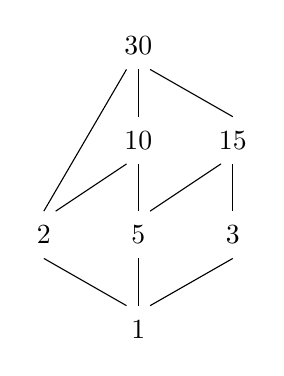
\begin{tikzpicture}[scale=0.6] %Replaced figure with tikz figure - TWJ 8/22/2010

\draw (0,0.5) -- (0,1.5);
\draw (0,2.5) -- (0,3.5);
\draw (2,2.5) -- (2,3.5);
\draw (0,4.5) -- (0,5.5);

\draw (0.25,5.5) -- (2,4.5);
\draw (-0.25,5.5) -- (-2,2.5);

\draw (1.75,3.5) -- (0.25,2.5);
\draw (-0.25,3.5) -- (-1.75,2.5);

\draw (2,1.5) -- (0.25,0.5);
\draw (-2,1.5) -- (-0.25,0.5);

\node at (0,6) {30};
\node at (0,4) {10};
\node at (2,4) {15};
\node at (-2, 2) {2};
\node at (0, 2) {5};
\node at (2, 2) {3};
\node at (0, 0) {1};

\end{tikzpicture}
\end{center}
 
 
 
\item[5.] 
False.
 

 
\item[6.]
(a) $(a \vee b \vee a') \wedge a$.
\begin{center}  
\tikzpreface{solution_circuit_a}
\begin{tikzpicture}[scale=0.8,node distance=5mm, text height=1.5ex,text depth=.25ex] %Replaced figure with tikz figure - TWJ 8/22/2010

\draw  (0,0) -- (2.2,0) (2.8,0) -- (4.7,0)  (5.3,0) -- (6,0);
\draw  (1,0) -- (1,1) -- (2.2,1)  (2.8,1) -- (4,1) -- (4,0);
\draw  (1,0) -- (1,-1) -- (2.2,-1)  (2.8,-1) -- (4,-1) -- (4,0);

\node at (2.5,-1) {$a'$};
\node at (2.5,0) {$b$};
\node at (2.5,1) {$a$};
\node at (5,0) {$a$};



\end{tikzpicture}
\end{center}
 


(c) $a \vee (a \wedge b)$.
\begin{center}  

\tikzpreface{solution_circuit_c}
\begin{tikzpicture}[scale=0.8,node distance=5mm, text height=1.5ex,text depth=.25ex] %Replaced figure with tikz figure - TWJ 8/22/2010

\draw  (0,0) -- (1,0) (4,0) -- (5,0);
\draw  (1,0) -- (1,1) -- (1.7,1)  (2.3,1) -- (2.7,1)  (3.3,1) -- (4,1) -- (4,0);
\draw  (1,0) -- (1,-1) -- (2.2,-1)  (2.8,-1) -- (4,-1) -- (4,0);

\node at (2.5,-1) {$a$};
\node at (2,1) {$a$};
\node at (3,1) {$b$};



\end{tikzpicture}
\end{center}
 
 
 
 
\item[8.]
Not equivalent.
 
\item[10.]
$a' \wedge [(a \wedge b') \vee b] = a \wedge (a \vee b)$.

\item[15.]
Let $I, J$ be ideals in $R$. We need to show that $I + J 
= \{ r + s : r \in
I \mbox{ and } s \in J  \}$ is the smallest ideal in $R$ containing
both $I$ and $J$. If $r_1, r_2 \in I$ and $s_1, s_2 \in J$, then
$(r_1 + s_1) + (r_2 + s_2) = (r_1 + r_2) +(s_1 + s_2)$ is in $I + J$.
For $a \in R$, $a(r_1 + s_1) = ar_1 + as_1 \in I + J$; hence, $I + J$
is an ideal in $R$.


\item[19.]
(a) No.

\item[21.]
$( \Rightarrow)$. $a = b \Rightarrow (a \wedge b') \vee (a' \wedge b)
= (a \wedge a') \vee (a' \wedge a) = O \vee O = O$. \\
$( \Leftarrow)$. $( a \wedge b') \vee (	a' \wedge b) = O \Rightarrow
a \vee b = (a \vee a) \vee b = a \vee (a \vee b) = a \vee [I \wedge
(a \vee b)] = a \vee [(a \vee a') \wedge (a \vee b)] = [a \vee
(a \wedge b')] \vee [a \vee (a' \wedge b)] = a \vee [(a \wedge b') \vee
(a' \wedge b)] = a \vee 0 = a$.  A symmetric argument shows that $a
\vee b = b$.



 
\end{itemize}
}
 
\subsection*{Chapter 20. Vector Spaces}
 
{\small
\begin{itemize}
 
\item[3.] 
${\mathbb Q}(\sqrt{2}, \sqrt{3}\, )$ has basis $\{ 1, \sqrt{2}, \sqrt{3},
\sqrt{6}\, \}$  over ${\mathbb Q}$.
 
\item[5.]
$P_n$ has basis $\{ 1, x, x^2, \ldots, x^{n-1} \}$.
 
\item[7.]
(a) Subspace of dimension 2 with basis $\{(1, 0, -3), (0, 1,
2) \}$.\\
(d) Not a subspace.
 
\item[10.]
$0 =  \alpha 0 = \alpha(-v+v) = \alpha(-v) + \alpha v \Rightarrow 
-\alpha v = \alpha(-v)$.
 
\item[12.]
Let $v_0 = 0, v_1, \ldots, v_n \in V$ and $\alpha_0 \neq 0, \alpha_1,
\ldots, \alpha_n \in F$. Then $\alpha_0 v_0 + \cdots + \alpha_n v_n =
0$.
 
\item[15.]
(a)
Let $u, v \in \ker(T)$ and $\alpha \in F$.  Then
\[
\begin{array}{c}
T(u +v) = T(u) + T(v) = 0 \\
T(\alpha v) = \alpha T(v) = \alpha 0 = 0.
\end{array}
\]
Hence, $u + v, \alpha v \in \ker(T) \Rightarrow \ker(T)$ is 
a subspace of
$V$. \\
(c) 
$T(u) = T(v) \Leftrightarrow T(u-v) = T(u) - T(v) = 0
\Leftrightarrow u-v = 0 \Leftrightarrow u = v$.
 
 
\item[17.]
(a)
Let $u, u' \in U$ and $v, v' \in V$. Then
\[
\begin{array}{c}
(u + v) + (u' + v') = (u + u') + (v + v') \in U + V \\
\alpha(u + v) = \alpha u + \alpha v \in U + V.
\end{array}
\]
 
\end{itemize}
}
 
\subsection*{Chapter 21. Fields}
 
{\small
\begin{itemize}
 
\item[1.] 
(a) $x^4 -\frac{2}{3} x^2 - \frac{62}{9}$.
(c) $x^4 - 2 x^2 + 25$.
 
\item[2.] 
(a) $\{ 1, \sqrt{2}, \sqrt{3}, \sqrt{6}\, \}$.
(c) $\{ 1, i, \sqrt{2}, \sqrt{2}\, i \}$.
(e) $\{1, 2^{1/6}, 2^{1/3}, 2^{1/2}, 2^{2/3}, 2^{5/6}  \}$.
 
\item[3.]
(a) ${\mathbb Q}(\sqrt{3}, \sqrt{7}\, )$.
 

\item[5.]
Use the fact that the elements of ${\mathbb Z}_2[x]/ \langle x^3 + x +
1\rangle$ are 0, 1, $\alpha$, $1 + \alpha$, $\alpha^2$, $1 + \alpha^2$,
$\alpha + \alpha^2$, $1 + \alpha + \alpha^2$ and the fact that
$\alpha^3 + \alpha + 1 = 0$. 


\item[8.]
False.


\item[14.]
Suppose that $E$ is algebraic over $F$ and $K$ is
algebraic over $E$. Let $\alpha \in K$. It suffices to show that
$\alpha$ is algebraic over some finite extension of $F$. Since
$\alpha$ is algebraic over $E$, it must be the zero of some polynomial
$p(x) = \beta_0 + \beta_1 x + \cdots + \beta_n x^n$ in $E[x]$. Hence
$\alpha$ is algebraic over $F(\beta_0, \ldots, \beta_n)$.


\item[22.]
${\mathbb Q}( \sqrt{3}, \sqrt{7}\, ) \supset {\mathbb Q}( \sqrt{3} +\sqrt{7}\,
)$ since $\{ 1, \sqrt{3}, \sqrt{7}, \sqrt{21}\, \}$ is a basis for
${\mathbb Q}( \sqrt{3}, \sqrt{7}\, )$ over ${\mathbb Q}$. Since $[{\mathbb Q}(
\sqrt{3}, \sqrt{7}\, ) : {\mathbb Q}] = 4$, $[{\mathbb Q}( \sqrt{3}
+\sqrt{7}\, ) : {\mathbb Q}] = 2$ or 4. Since the degree of the minimal
polynomial of $\sqrt{3} +\sqrt{7}$ is 4, ${\mathbb Q}( \sqrt{3},
\sqrt{7}\, ) = {\mathbb Q}( \sqrt{3} +\sqrt{7}\, )$.


\item[27.]
Let $\beta \in F(\alpha)$ not in $F$. Then $\beta =
p(\alpha)/q(\alpha)$, where $p$ and $q$ are polynomials in $\alpha$
with $q(\alpha) \neq 0$ and coefficients in $F$. If $\beta$ is
algebraic over $F$, then there exists a polynomial $f(x) \in F[x]$
such that $f(\beta) = 0$. Let $f(x) = a_0 + a_1 x + \cdots + a_n x^n$.
Then  
\[
0 = f(\beta) = f\left( 
\frac{p(\alpha)}{q(\alpha)} \right)
= a_0 + a_1 \left( \frac{p(\alpha)}{q(\alpha)} \right)  + \cdots + a_n
\left( \frac{p(\alpha)}{q(\alpha)} \right)^n. 
\]
Now multiply both sides by $q(\alpha)^n$ to show that there is a
polynomial in $F[x]$ that has $\alpha$ as a zero.




\end{itemize}
}
 
\subsection*{Chapter 22. Finite Fields}
 
{\small
\begin{itemize}

\item[1.]
(a) 2.
(c) 2.
 
\item[4.] 
There are eight elements in ${\mathbb Z}_2(\alpha)$. Exhibit two more
zeros of $x^3 + x^2 + 1$ other than $\alpha$ in these eight elements. 
 
\item[5.] 
Find an irreducible polynomial $p(x)$ in ${\mathbb Z}_3[x]$ of degree
3 and show that ${\mathbb Z}_3[x]/ \langle p(x) \rangle$ has 27
elements. 

\item[7.]
(a) $x^5 -1 = (x+1)(x^4+x^3 + x^2 + x+ 1)$. \\
(c) $x^9 -1 = (x+1)( x^2 + x+ 1)(x^6+x^3+1)$.
 
\item[8.]
True.

\item[11.]
(a) Use the fact that $x^7 -1 = (x+1)( x^3 + x+ 1)(x^3+x^2+1)$.

\item[12.]
False.

\item[17.]
If $p(x) \in F[x]$, then $p(x) \in E[x]$.


\item[18.]
Since $\alpha$ is algebraic over $F$ of degree $n$, we can write any
element $\beta \in F(\alpha)$ uniquely as $\beta = a_0  + a_1 \alpha +
\cdots + a_{n-1} \alpha^{n-1}$ with $a_i \in F$. There are $q^n$
possible $n$-tuples $(a_0, a_1, \ldots, a_{n-1})$.


\item[24.]
Factor $x^{p-1} - 1$ over ${\mathbb Z}_p$.


\end{itemize}
}
 
\subsection*{Chapter 23. Galois Theory}
 
{\small
\begin{itemize}
 
\item[1.]
(a) ${\mathbb Z}_2$.
(c) ${\mathbb Z}_2 \times {\mathbb Z}_2 \times {\mathbb Z}_2$.
 
\item[2.]
(a) Separable.
(c) Not separable.
 
\item[3.]
$[{\rm GF}(729): {\rm GF}(9)] = [{\rm GF}(729): {\rm GF}(3)] /[{\rm
GF}(9): {\rm GF}(3)] = 6/2 = 3 \Rightarrow G({\rm GF}(729)/ {\rm
GF}(9)) \cong {\mathbb Z}_3$. A generator for $G({\rm GF}(729)/ {\rm
GF}(9))$ is $\sigma$, where $\sigma_{3^6}( \alpha) = \alpha^{3^6} =
\alpha^{729}$ for $\alpha \in {\rm GF}(729)$.

\item[4.]
(a) $S_5$.
(c) $S_3$.

\item[5.]
(a) ${\mathbb Q}(i)$.


\item[7.]
Let $E$ be the splitting field of a cubic polynomial in $F[x]$. Show that
\mbox{$[E:F]$} is less than or equal to 6 and is divisible by 3. Since $G(E/F)$ is a subgroup of
$S_3$ whose order is divisible by 3, conclude that this group must be 
isomorphic to ${\mathbb Z}_3$ or $S_3$.
 
\item[9.]
$G$ is a subgroup of $S_n$.

\item[16.]
True.

\item[20.]
(a) Clearly $\omega, \omega^2, \ldots, \omega^{p-1}$ are
distinct since $\omega \neq 1$ or 0. To show that $\omega^i$ is a zero
of $\Phi_p$, calculate $\Phi_p( \omega^i)$. \\
(b) The conjugates of $\omega$ are $\omega, \omega^2, \ldots,
\omega^{p-1}$. Define a map  $\phi_i: {\mathbb Q}(\omega)
\rightarrow {\mathbb Q}(\omega^i)$ by 
\[
\phi_i(a_0 + a_1 \omega +
\cdots + a_{p-2} \omega^{p-2}) = a_0 + a_1 \omega^i + \cdots + c_{p-2} 
(\omega^i)^{p-2},
\]
where $a_i \in {\mathbb Q}$. Prove that $\phi_i$ is an isomorphism of
fields. Show that $\phi_2$ 
generates $G({\mathbb Q}(\omega)/{\mathbb Q})$. \\ 
(c)
Show that $\{ \omega, \omega^2, \ldots, \omega^{p-1} \}$ is a basis
for ${\mathbb Q}( \omega )$ over ${\mathbb Q}$, and consider which linear
combinations of $\omega, \omega^2, \ldots, \omega^{p-1}$ are left
fixed by all elements of $G( {\mathbb Q}( \omega ) / {\mathbb Q})$.
 
 
 
\end{itemize}
}
 
 
 
 
\pagestyle{headings}
 
 
 
 
